\chapter {Analysis on players data}

Analysis are performed on different abstraction levels.

At the beginning, high-level evaluations are made to discover stats on number of played matches (mean, min, max etc.); analysis on number of played matches are reported in figure \ref{fig:countMatch}.
\\
\begin{figure}[H]
  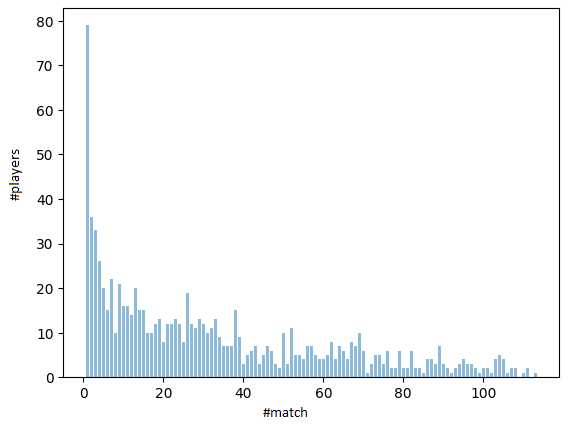
\includegraphics[scale=0.9]{images/img-01.png}
   \caption{\textit{Count number of players that played a certain number of matches.}}
  \label{fig:countMatch}
\end{figure}

Similarly, a fine grained analysis has been made by grouping players per role, as shown in figure \ref{fig:countMatchPerRole}, but no relevant differences have been found.

\begin{figure}[H]
  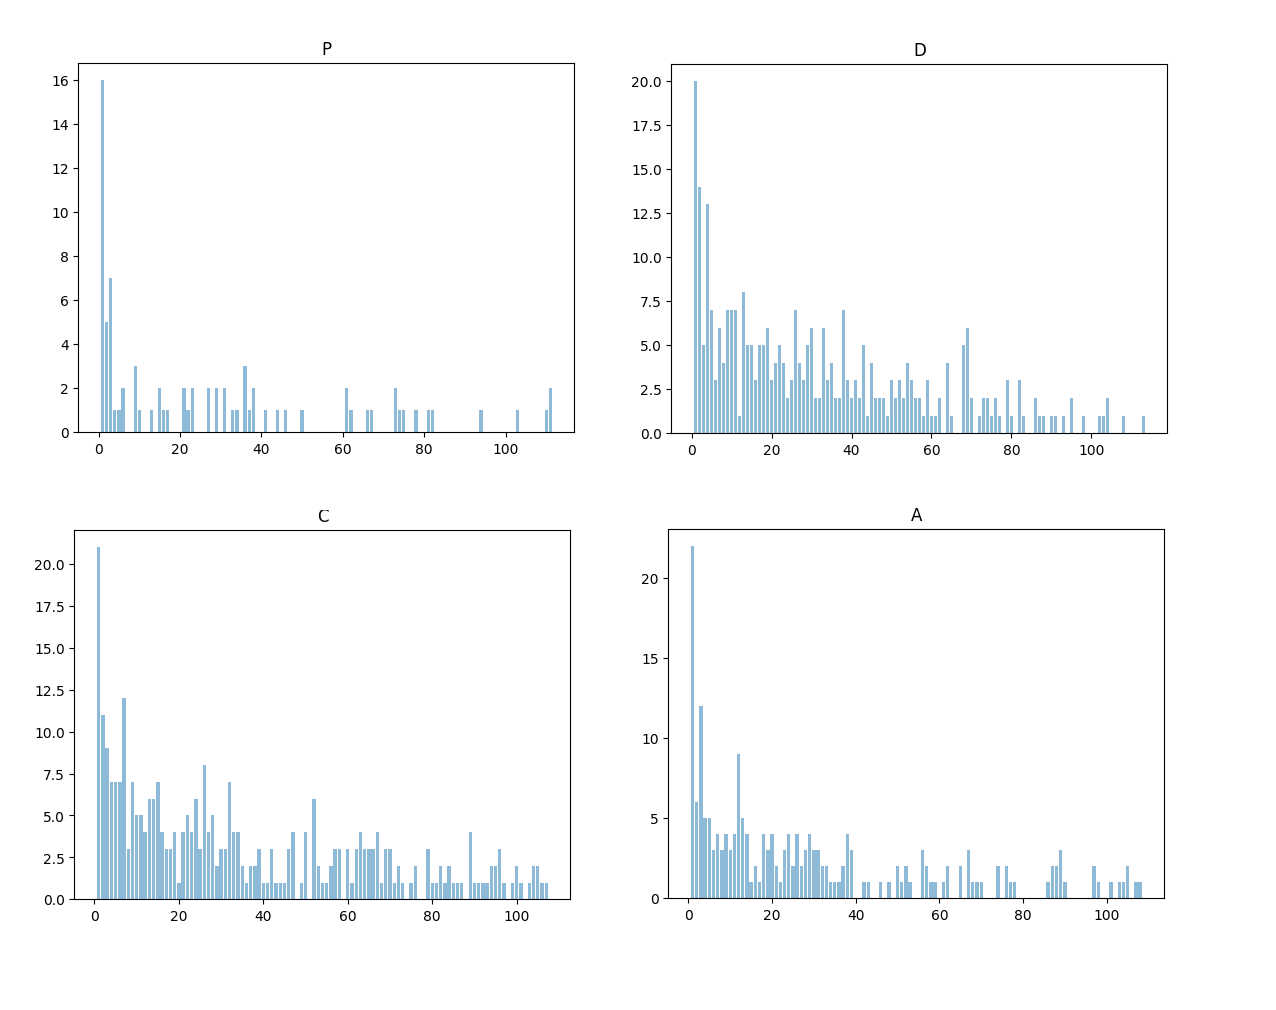
\includegraphics[scale=0.4]{images/img-02.png}
   \caption{\textit{Count number of players of such role that played a certain number of matches.
   Legend: P = Goalkeeper, D = Defender, C = Midfielder, A = Striker}}
  \label{fig:countMatchPerRole}
\end{figure}

\newpage
\section{Data correlation}

The task goal is discovering, if present, seasonality on players' votes.
\\
In order to achieve such a target, Pearson Correlation Index has been us, for single player and for role both.
\\
Empirical tests show that no relevant seasonality can be detected.
\\
Figure \ref{fig:playereg} reports data on an example player.

\begin{figure}[H]
  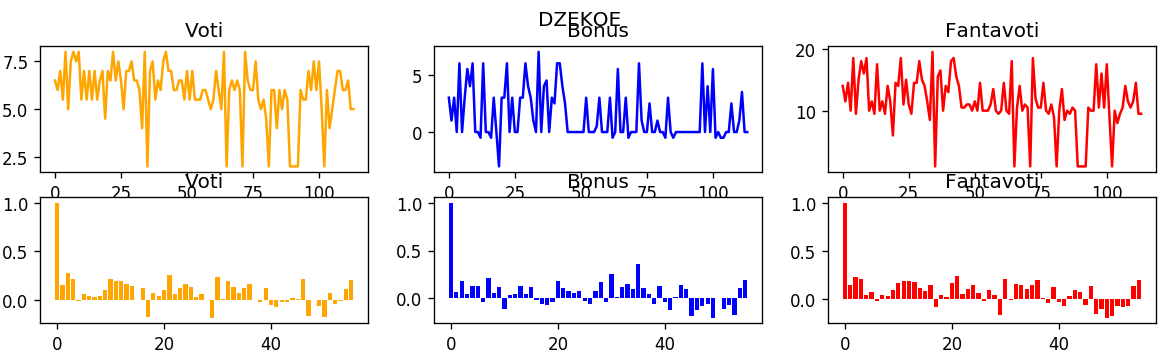
\includegraphics[scale=0.5]{images/img-03.png}
   \caption{\textit{The image shows storic series and respective Pearson correlations for ''Edin Dzeko''.}}
  \label{fig:playereg}
\end{figure}

\section{Normality test}


  